\documentclass[aspectratio=169]{beamer}
\usepackage[utf8]{inputenc}
\usepackage[spanish]{babel}
\usepackage{graphicx}
\usepackage{xcolor}
\usepackage{tikz}
\usetikzlibrary{arrows.meta, positioning, shapes}

% Tema oscuro personalizado
\definecolor{darkbg}{HTML}{0f172a}
\definecolor{lightgreen}{HTML}{deff9a}
\definecolor{lightblue}{HTML}{7dd3fc}
\definecolor{lightred}{HTML}{fca5a5}
\definecolor{textgray}{HTML}{cbd5e1}

\setbeamercolor{background canvas}{bg=darkbg}
\setbeamercolor{normal text}{fg=white}
\setbeamercolor{frametitle}{fg=lightgreen}
\setbeamercolor{title}{fg=white}
\setbeamercolor{itemize item}{fg=lightgreen}
\setbeamercolor{itemize subitem}{fg=lightblue}

\setbeamertemplate{navigation symbols}{}
\setbeamertemplate{footline}[frame number]

\title{Paralelización de KNN con MPI}
\subtitle{Optimización de algoritmos de Machine Learning utilizando modelos de paso de mensajes}
\author{Fabián Alvarado Ramos \\ Eduardo Miguel Salas Palacios \\ Neftalí Calixto Rojas}
\institute{Proyecto Universitario de Computación Paralela}
\date{}

\begin{document}

% Slide 1: Título
\begin{frame}
\titlepage
\end{frame}

% Slide 2: Introducción
\begin{frame}{Introducción: Reto y Solución}
\begin{columns}[T]
\column{0.5\textwidth}
\textbf{\color{lightgreen}1. ¿Qué es KNN?}
\begin{itemize}
    \item Algoritmo supervisado que clasifica datos según la mayoría de votos de sus vecinos cercanos.
\end{itemize}

\vspace{0.5cm}
\textbf{\color{lightgreen}2. El Problema (Cuello de Botella)}
\begin{itemize}
    \item Calcular distancias contra \textbf{todo} el dataset es costoso: $O(N \times M)$.
\end{itemize}

\vspace{0.5cm}
\textbf{\color{lightgreen}3. La Solución Propuesta}
\begin{itemize}
    \item Paralelizar el cálculo usando \textbf{MPI} y el modelo SPMD para dividir la carga entre múltiples procesadores.
\end{itemize}

\column{0.5\textwidth}
\centering
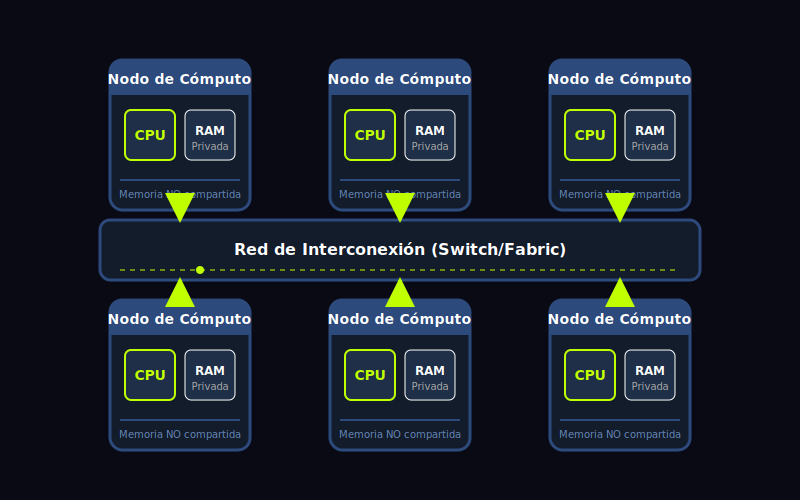
\includegraphics[width=\textwidth,height=0.6\textheight,keepaspectratio]{images/topologia}
\end{columns}
\end{frame}

% Slide 3: Metodología DAG
\begin{frame}{Metodología (Topología DAG)}
\begin{columns}[T]
\column{0.5\textwidth}
\textbf{\color{lightgreen}Arquitectura Maestro-Trabajador}

La paralelización se modela como un grafo de tareas dirigido:
\begin{itemize}
    \item \textbf{Inicio (Main):} El nodo maestro divide el dataset (Scatter).
    \item \textbf{Paralelo (T1-T4):} Cada trabajador calcula distancias en su fragmento de datos localmente.
    \item \textbf{Fin (End):} Se recolectan los resultados parciales (Gather) para la decisión final.
\end{itemize}

\column{0.5\textwidth}
\centering
\begin{tikzpicture}[scale=0.8, transform shape]
    \node[circle, draw=lightgreen, fill=darkbg, minimum size=1cm] (main) at (0,0) {Main};
    \node[circle, draw=lightgreen, fill=darkbg, minimum size=0.8cm] (t1) at (-3,-2) {T1};
    \node[circle, draw=lightgreen, fill=darkbg, minimum size=0.8cm] (t2) at (-1,-2) {T2};
    \node[circle, draw=lightgreen, fill=darkbg, minimum size=0.8cm] (t3) at (1,-2) {T3};
    \node[circle, draw=lightgreen, fill=darkbg, minimum size=0.8cm] (t4) at (3,-2) {T4};
    \node[circle, draw=lightblue, fill=darkbg, minimum size=1cm] (end) at (0,-4) {End};
    
    \draw[->, lightgreen, thick] (main) -- (t1);
    \draw[->, lightgreen, thick] (main) -- (t2);
    \draw[->, lightgreen, thick] (main) -- (t3);
    \draw[->, lightgreen, thick] (main) -- (t4);
    
    \draw[->, lightblue, thick] (t1) -- (end);
    \draw[->, lightblue, thick] (t2) -- (end);
    \draw[->, lightblue, thick] (t3) -- (end);
    \draw[->, lightblue, thick] (t4) -- (end);
    
    \node[textgray] at (-2,-1) {Scatter};
    \node[textgray] at (2,-3) {Gather};
\end{tikzpicture}
\end{columns}
\end{frame}

% Slide 4: Metodología Timeline
\begin{frame}{Metodología: Flujo de Ejecución}
\begin{center}
\begin{tikzpicture}[scale=1.2]
    \foreach \x/\label in {0/Beta 1: Scatter, 4/Beta 2: Broadcast, 8/Versión Final: Gather} {
        \node[circle, draw=lightgreen, fill=darkbg, minimum size=0.5cm] at (\x,0) {};
        \node[below=0.3cm, text width=3cm, align=center] at (\x,0) {\small\color{lightgreen}\textbf{\label}};
    }
    \draw[lightgreen, thick] (0,0) -- (8,0);
\end{tikzpicture}
\end{center}

\vspace{0.5cm}
\begin{columns}[T]
\column{0.33\textwidth}
\textbf{\color{lightgreen}Beta 1}
\begin{itemize}
    \item El nodo maestro lee los datos y utiliza \texttt{MPI\_Scatter} para distribuir fragmentos equitativos del dataset de prueba.
\end{itemize}

\column{0.33\textwidth}
\textbf{\color{lightgreen}Beta 2}
\begin{itemize}
    \item Se utiliza \texttt{MPI\_Bcast} para enviar el dataset de entrenamiento completo a todos los nodos.
\end{itemize}

\column{0.33\textwidth}
\textbf{\color{lightgreen}Versión Final}
\begin{itemize}
    \item El maestro recolecta todas las predicciones parciales usando \texttt{MPI\_Gather}.
\end{itemize}
\end{columns}
\end{frame}

% Slide 5: Topología del Clúster
\begin{frame}{Topología del Clúster}
\begin{columns}[T]
\column{0.5\textwidth}
La arquitectura implementada simula un entorno de memoria distribuida.

\begin{itemize}
    \item \textbf{Nodo 0 (Master):} Orquestador de I/O y recolección.
    \item \textbf{Nodos 1-N (Workers):} Motores de cálculo puro.
    \item \textbf{Comunicación:} Minimización de latencia mediante envío de bloques contiguos.
\end{itemize}

\column{0.5\textwidth}
\centering
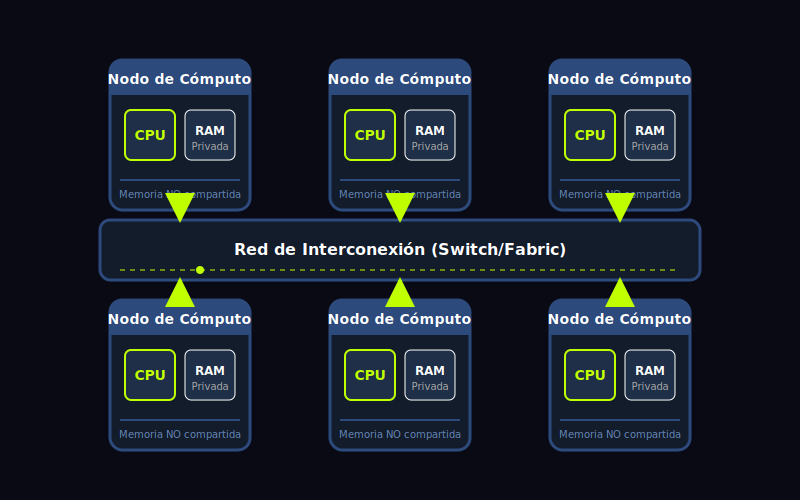
\includegraphics[width=\textwidth,height=0.6\textheight,keepaspectratio]{images/topologia}
\end{columns}
\end{frame}

% Slide 6: Resultados Precisión
\begin{frame}{Resultados: Validación del Algoritmo}
\begin{center}
\Huge\color{lightgreen}\textbf{0.9833}

\vspace{0.5cm}
\Large Precisión (Accuracy)

\vspace{1cm}
\normalsize\color{textgray}
Idéntica a la versión secuencial.\\
Garantía de corrección en el cálculo paralelo.
\end{center}
\end{frame}

% Slide 7: Tiempo de Ejecución
\begin{frame}{Rendimiento: Tiempo de Ejecución}
\begin{columns}[T]
\column{0.5\textwidth}
\begin{itemize}
    \item \textbf{Reducción drástica:} El tiempo baja de 5s a casi 2s al pasar de 1 a 4 procesos.
    \item \textbf{Punto de Saturación:} Observa el "codo" en 4 procesos. Añadir más nodos (8) apenas mejora el tiempo.
    \item \textbf{Causa:} El tiempo de comunicación empieza a pesar más que el ahorro en cálculo.
\end{itemize}

\column{0.5\textwidth}
\centering
\includegraphics[width=\textwidth,height=0.7\textheight,keepaspectratio]{images/time_vs_processes.png}
\end{columns}
\end{frame}

% Slide 8: Speedup
\begin{frame}{Análisis de Aceleración (Speedup)}
\begin{columns}[T]
\column{0.5\textwidth}
\begin{itemize}
    \item \textbf{Ideal vs Real:} La línea punteada es el ideal. Nuestra curva real se aleja al aumentar N.
    \item \textbf{Speedup Máximo:} Logramos acelerar 2.5x veces el proceso con 8 nodos.
    \item \textbf{Ley de Amdahl:} La parte secuencial del código (I/O y envíos) limita la velocidad máxima teórica.
\end{itemize}

\column{0.5\textwidth}
\centering
\includegraphics[width=\textwidth,height=0.7\textheight,keepaspectratio]{images/speedup.png}
\end{columns}
\end{frame}

% Slide 9: Eficiencia
\begin{frame}{Eficiencia del Clúster}
\begin{columns}[T]
\column{0.5\textwidth}
\begin{itemize}
    \item \textbf{Caída de Eficiencia:} Del 94\% (excelente) con 2 nodos, bajamos al 31\% con 8 nodos.
    \item \textbf{¿Qué significa?} Con 8 nodos, estamos desperdiciando el 70\% de la capacidad de CPU en esperas.
    \item \textbf{Conclusión:} Para este tamaño de dataset, 4 nodos es la configuración más rentable (60\% eficiencia).
\end{itemize}

\column{0.5\textwidth}
\centering
\includegraphics[width=\textwidth,height=0.7\textheight,keepaspectratio]{images/efficiency.png}
\end{columns}
\end{frame}

% Slide 10: FLOPs
\begin{frame}{Rendimiento (GFLOPs)}
\begin{columns}[T]
\column{0.5\textwidth}
\begin{itemize}
    \item \textbf{Potencia Bruta:} A pesar de la ineficiencia, la cantidad total de operaciones por segundo sube.
    \item \textbf{Escalabilidad Fuerte:} El sistema es capaz de entregar más cómputo si se le exige más.
    \item \textbf{Utilidad:} Esto justifica el uso del clúster si el dataset creciera de 8k a 1 millón de datos.
\end{itemize}

\column{0.5\textwidth}
\centering
\includegraphics[width=\textwidth,height=0.7\textheight,keepaspectratio]{images/flops.png}
\end{columns}
\end{frame}

% Slide 11: Escalabilidad
\begin{frame}{Escalabilidad del Problema (Datos)}
\begin{columns}[T]
\column{0.5\textwidth}
\begin{itemize}
    \item \textbf{Configuración:} Se mantuvo fijo el clúster en 4 procesadores (p=4) y se varió el tamaño del dataset (N).
    \item \textbf{Crecimiento Cuadrático:} Al duplicar N (de 4k a 8k), el tiempo se triplica (18s a 67s), confirmando la complejidad $O(N^2)$.
    \item \textbf{Límite:} El sistema puede manejar datasets más grandes, pero el tiempo crecerá exponencialmente.
\end{itemize}

\column{0.5\textwidth}
\centering
\includegraphics[width=\textwidth,height=0.7\textheight,keepaspectratio]{images/scalability_n.png}
\end{columns}
\end{frame}

% Slide 12: Conclusiones
\begin{frame}{Conclusiones del Proyecto}
\begin{itemize}
    \item[\color{lightblue}✓] \textbf{Paralelización Exitosa:} Reducción del tiempo de 5.02s a 2.01s. El algoritmo es correcto y más rápido.
    
    \vspace{0.5cm}
    \item[\color{lightgreen}✓] \textbf{Punto Óptimo:} Con 4 procesos se obtiene el mejor balance entre Speedup (2.4x) y Eficiencia (60\%).
    
    \vspace{0.5cm}
    \item[\color{lightred}⚠] \textbf{Cuello de Botella:} Con 8 procesos, la ganancia es marginal debido al costo de comunicación, y con grandes datasets el tiempo crece cuadráticamente.
\end{itemize}
\end{frame}

% Slide 13: Q&A
\begin{frame}
\begin{center}
\Huge\color{lightgreen}¿Preguntas?

\vspace{1cm}
\Large Gracias por su atención

\vspace{1cm}
\normalsize Proyecto KNN con MPI
\end{center}
\end{frame}

\end{document}
